\documentclass[letterpaper,landscape]{article} 
\usepackage[english]{babel}
\usepackage{natbib} 
\usepackage[official]{eurosym}
\usepackage{float} 
\usepackage[a4paper, margin=0.2in]{geometry}

% general utils
\newcommand{\comment}[1]{}

% remove page numbers
\pagenumbering{gobble}

% math
\usepackage{xfrac}
\usepackage{amssymb,amsmath,amsfonts,amsthm}
\newcommand{\parenthesis}[1]{\left(#1\right)}

\usepackage{xcolor}
\usepackage{colortbl}

% figures and tikz
\usepackage{pgf}
\usepackage{pgfplots}
\usepackage{tikz}
\pgfplotsset{compat=newest}
\usepgfplotslibrary{polar}
\usetikzlibrary{fit,calc,arrows,positioning,shapes,decorations.pathreplacing,matrix}


\def\rowheight{0.35}
\def\namewidth{4.1}
\def\unknowncolor{white}
\def\nonecolor{black!90}
\def\rarecolor{red!40}
\def\uncommoncolor{yellow!50}
\def\commoncolor{green!40}
\def\nestingcolor{black!90}
\def\monthtextoptions{\small \bf}
\def\monthtextoptionsdig{\footnotesize \bf }
\def\monthtxtoffset{0.55}

% NOTE: by convention positions refer to the left side of the whole row

% -- box for ticking observation (\rowheight by \rowheight)
\newcommand{\drawtickingbox}[2]{% {x}{y}
  \draw[black!90] (#1,#2) rectangle ++(\rowheight,\rowheight);
}

% -- box where the name of the bird will appear (\namewidth by \rowheight)
\newcommand{\drawnamebox}[2]{% {x}{y}
  \draw[black!90] (\rowheight+#1,#2) rectangle ++(\namewidth,\rowheight);
}

% -- write the name of the bird (kind of depends on \rowheight being 0.35)
\newcommand{\birdname}[3]{%
  \node[anchor=base,label=right:{\small #3}] () at (0.5*\rowheight+#1,0.45*\rowheight+#2) {};      
}

% -- draw the nesting sign for a single digit month (this time x,y are in absolute reference)
\newcommand{\drawnestingsign}[2]{% {x}{y}
  \begin{scope}[shift={(#1,#2)}]
    \draw[fill=\nestingcolor] (0,0) -- (0.5*\rowheight,0) to[out=180,in=-90] (0,0.5*\rowheight)  -- cycle;
    \draw[fill=\nestingcolor] (0.5*\rowheight,0) -- (\rowheight,0) -- (\rowheight,0.5*\rowheight) to[out=-90,in=0] cycle;
    \draw[fill=\nestingcolor] (0,\rowheight) -- (0.5*\rowheight,\rowheight) to[out=180,in=90] (0,0.5*\rowheight)  -- cycle;
    \draw[fill=\nestingcolor] (0.5*\rowheight,\rowheight) -- (\rowheight,\rowheight) -- (\rowheight,0.5*\rowheight) to[out=90,in=0] cycle;
  \end{scope}
}

% -- draw the nesting sign for a double digit month (this time x,y are in absolute reference)
\newcommand{\drawnestingsigndig}[2]{% {x}{y}
  \begin{scope}[shift={(#1,#2)}]
    \draw[fill=\nestingcolor] (0,0) -- (0.5*1.2*\rowheight,0) to[out=180,in=-90] (0,0.5*\rowheight)  -- cycle;
    \draw[fill=\nestingcolor] (0.5*1.2*\rowheight,0) -- (1.2*\rowheight,0) -- (1.2*\rowheight,0.5*\rowheight)  to[out=-90,in=0] cycle;
    \draw[fill=\nestingcolor] (0,\rowheight) -- (0.5*1.2*\rowheight,\rowheight) to[out=180,in=90] (0,0.5*\rowheight)  -- cycle;
    \draw[fill=\nestingcolor] (0.5*1.2*\rowheight,\rowheight) -- (1.2*\rowheight,\rowheight) -- (1.2*\rowheight,0.5*\rowheight) to[out=90,in=0] cycle;
  \end{scope}
}

% -- draw the box for a single month (this time x,y are in absolute reference)
% Observation Key conventions:
% unknown             := 0
% common              := 1
% common-nesting      := 2
% uncommon            := 3
% uncommon-nesting    := 4
% rare                := 5
% rare-nesting        := 6
% none                := 7
%\def\monthcolorslist{{\nonecolor,\commoncolor,\commoncolor,\uncommoncolor,\uncommoncolor,\rarecolor,\rarecolor}}
% had to be set manually ...
\def\monthcolorslist{{"white","green!40","green!40","yellow!50","yellow!50","red!40","red!40","black!90"}}
\newcommand{\drawmonthbox}[4]{% {x}{y}{observationKey}{monthDigBoolean}
  \begin{scope}[shift={(#1,#2)}]
  \def\myindex{#3} % figure out the color
  \pgfmathparse{\monthcolorslist[\myindex]}
  \edef\mycolor{\pgfmathresult}
  \ifnum#4=0{ % single digit month
    \draw[black!90,fill={\mycolor}] (0,0) rectangle ++(\rowheight,\rowheight);
    \ifnum#3=2{ \drawnestingsign{0}{0} }\fi
    \ifnum#3=4{ \drawnestingsign{0}{0} }\fi
    \ifnum#3=6{ \drawnestingsign{0}{0} }\fi
  }\fi
  \ifnum#4=1{ % double digit month
    \draw[black!90,fill={\mycolor}] (0,0) rectangle ++(1.2*\rowheight,\rowheight);
    \ifnum#3=2{ \drawnestingsigndig{0}{0} }\fi
    \ifnum#3=4{ \drawnestingsigndig{0}{0} }\fi
    \ifnum#3=6{ \drawnestingsigndig{0}{0} }\fi
  }\fi
  \end{scope}
}

% -- draw month boxes given a list of observation keys for all 12 months
\newcommand{\drawmonthboxes}[1]{% {observationKeyList}
  \foreach \obskey [count=\month] in #1 {
    \ifnum\month<10{ % single digit months
      \pgfmathparse{(\month)*\rowheight}
      \drawmonthbox{\namewidth+\pgfmathresult}{0}{\obskey}{0}
    }\fi
    \ifnum\month>9{ % double digit months
      \pgfmathparse{(\month+0.2*(\month-10))*\rowheight}
      \drawmonthbox{\namewidth+\pgfmathresult}{0}{\obskey}{1}
    }\fi
  }
}

% -- write the labels for each months in numbers (kind of depends on \rowheight being 0.35)
\newcommand{\monthslabels}[2]{% {x}{y}
  \begin{scope}[shift={(#1,#2)}]
    \foreach \month in {1, 2, ..., 12}{
      \ifnum\month<10{
        \pgfmathparse{(0.55+\month-1)*\rowheight}
        \node[anchor=base,label=right:{\monthtextoptions \month}] () at (\namewidth+\pgfmathresult,\rowheight/2) {};
      }\fi
      \ifnum\month=10{
        \node[anchor=base,label=right:{\monthtextoptionsdig \month}] () at (\namewidth+9.35*\rowheight,\rowheight/2) {};
      }\fi
      \ifnum\month=11{
        \node[anchor=base,label=right:{\monthtextoptionsdig \month}] () at (\namewidth+10.58*\rowheight,\rowheight/2) {};
      }\fi
      \ifnum\month=12{
        \node[anchor=base,label=right:{\monthtextoptionsdig \month}] () at (\namewidth+11.78*\rowheight,\rowheight/2) {};
      }\fi
    }
  \end{scope}
}

% -- top level function for bird box!
\newcommand{\drawbirdbox}[4]{% {x}{y}{name}{observationKeyList}
  \begin{scope}[shift={(#1,#2)}]
    \drawtickingbox{0}{0}
    \drawnamebox{0}{0}
    \birdname{0}{0}{#3}
    \drawmonthboxes{#4}
    \monthslabels{0}{0}
  \end{scope}
}

\newcommand{\drawlegend}[2]{% {x}{y}
  \begin{scope}[shift={(#1+0.3*\rowheight,#2)}]
    \begin{scope}[shift={(0,0)}]
      \drawmonthbox{0}{0}{0}{0}
      \node[anchor=base,label=right:{\footnotesize Unknown}] () at (0.5*\rowheight,0.45*\rowheight) {};      
    \end{scope}
    \begin{scope}[shift={(1*1.8+0.15,0)}]
      \drawmonthbox{0}{0}{1}{0}
      \node[anchor=base,label=right:{\footnotesize Common}] () at (0.5*\rowheight,0.45*\rowheight) {};      
    \end{scope}
    \begin{scope}[shift={(2*1.8+0.15,0)}]
      \drawmonthbox{0}{0}{3}{0}
      \node[anchor=base,label=right:{\footnotesize Uncommon}] () at (0.5*\rowheight,0.45*\rowheight) {};      
    \end{scope}
    \begin{scope}[shift={(3*1.8+0.5,0)}]
      \drawmonthbox{0}{0}{5}{0}
      \node[anchor=base,label=right:{\footnotesize Rare}] () at (0.5*\rowheight,0.45*\rowheight) {};      
    \end{scope}
    \begin{scope}[shift={(4*1.8,0)}]
      \drawmonthbox{0}{0}{0}{0}
      \drawnestingsign{0}{0}
      \node[anchor=base,label=right:{\footnotesize Nesting}] () at (0.5*\rowheight,0.45*\rowheight) {};      
    \end{scope}
  \end{scope}
}

\begin{document}

\begin{center}
  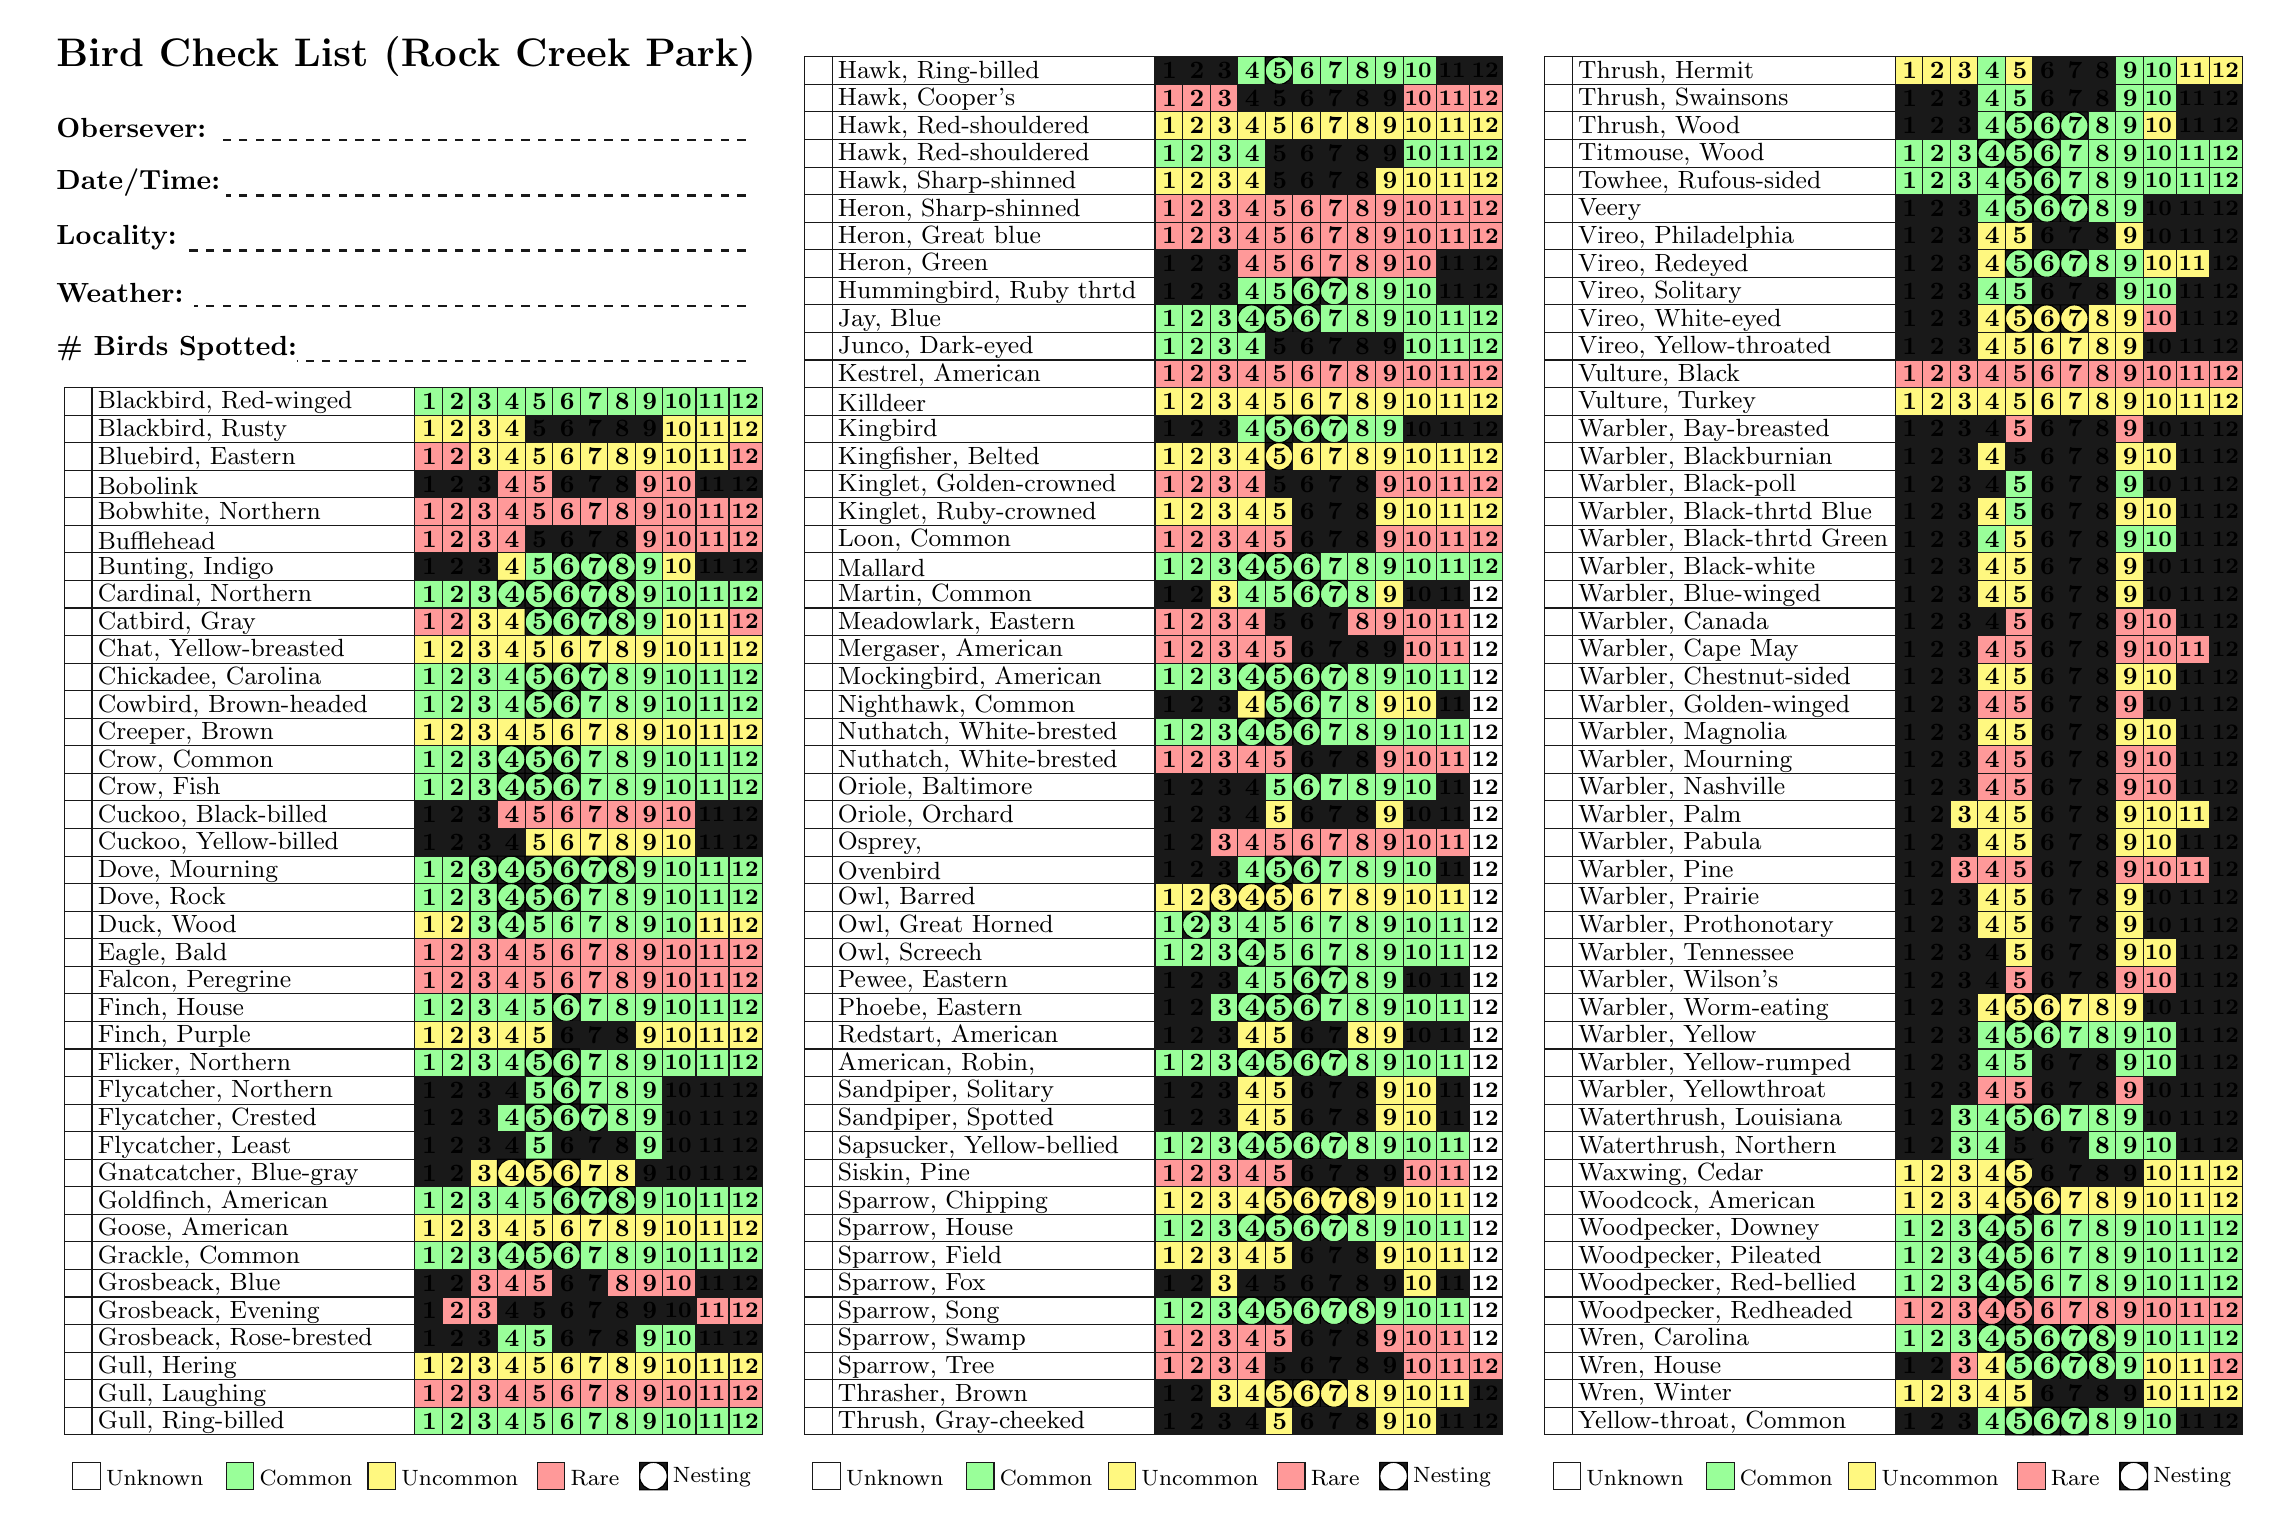
\begin{tikzpicture}[>=latex]
    \begin{scope}[shift={(0,0)}]
      \node[anchor=base,label=right:{\Large \bf Bird Check List (Rock Creek Park)}] () at (-\rowheight,\rowheight) {};      
      \begin{scope}[shift={(-\rowheight,0.15)}]
        \def\linedist{0.7}
        \node[anchor=base,label=right:{\bf Obersever:}] () at (0,-1*\linedist) {};
        \draw[thick,black!90,dashed] (9,-0.16-1*\linedist) -- ++(-6.7,0);
        \node[anchor=base,label=right:{\bf Date/Time:}] () at (0,-2*\linedist) {};
        \draw[thick,black!90,dashed] (9,-0.16-2*\linedist) -- ++(-6.6,0);
        \node[anchor=base,label=right:{\bf Locality:}] () at (0,-3*\linedist) {};
        \draw[thick,black!90,dashed] (9,-0.16-3*\linedist) -- ++(-7.1,0);
        \node[anchor=base,label=right:{\bf Weather:}] () at (0,-4*\linedist) {};
        \draw[thick,black!90,dashed] (9,-0.16-4*\linedist) -- ++(-7,0);
        \node[anchor=base,label=right:{\bf \# Birds Spotted:}] () at (0,-5*\linedist) {};
        \draw[thick,black!90,dashed] (9,-0.16-5*\linedist) -- ++(-5.7,0);
      \end{scope}
      \begin{scope}[shift={(0,-12*\rowheight)}]
        \drawbirdbox{0}{-0 * \rowheight}{Blackbird, Red-winged}{{1,1,1,1,1,1,1,1,1,1,1,1}};
        \drawbirdbox{0}{-1 * \rowheight}{Blackbird, Rusty}{{3,3,3,3,7,7,7,7,7,3,3,3}};
        \drawbirdbox{0}{-2 * \rowheight}{Bluebird, Eastern}{{5,5,3,3,3,3,3,3,3,3,3,5}};
        \drawbirdbox{0}{-3 * \rowheight}{Bobolink}{{7,7,7,5,5,7,7,7,5,5,7,7}};
        \drawbirdbox{0}{-4 * \rowheight}{Bobwhite, Northern}{{5,5,5,5,5,5,5,5,5,5,5,5}};
        \drawbirdbox{0}{-5 * \rowheight}{Bufflehead }{{5,5,5,5,7,7,7,7,5,5,5,5}};
        \drawbirdbox{0}{-6 * \rowheight}{Bunting, Indigo}{{7,7,7,3,1,2,2,2,1,3,7,7}};
        \drawbirdbox{0}{-7 * \rowheight}{Cardinal, Northern}{{1,1,1,2,2,2,2,2,1,1,1,1}};
        \drawbirdbox{0}{-8 * \rowheight}{Catbird, Gray}{{5,5,3,3,2,2,2,2,1,3,3,5}};
        \drawbirdbox{0}{-9 * \rowheight}{Chat, Yellow-breasted}{{3,3,3,3,3,3,3,3,3,3,3,3}};
        \drawbirdbox{0}{-10 * \rowheight}{Chickadee, Carolina}{{1,1,1,1,2,2,2,1,1,1,1,1}};
        \drawbirdbox{0}{-11 * \rowheight}{Cowbird, Brown-headed}{{1,1,1,1,2,2,1,1,1,1,1,1}};
        \drawbirdbox{0}{-12 * \rowheight}{Creeper, Brown}{{3,3,3,3,3,3,3,3,3,3,3,3}};
        \drawbirdbox{0}{-13 * \rowheight}{Crow, Common}{{1,1,1,2,2,2,1,1,1,1,1,1}};
        \drawbirdbox{0}{-14 * \rowheight}{Crow, Fish}{{1,1,1,2,2,2,1,1,1,1,1,1}};
        \drawbirdbox{0}{-15 * \rowheight}{Cuckoo, Black-billed}{{7,7,7,5,5,5,5,5,5,5,7,7}};
        \drawbirdbox{0}{-16 * \rowheight}{Cuckoo, Yellow-billed}{{7,7,7,7,3,3,3,3,3,3,7,7}};
        \drawbirdbox{0}{-17 * \rowheight}{Dove, Mourning}{{1,1,2,2,2,2,2,2,1,1,1,1}};
        \drawbirdbox{0}{-18 * \rowheight}{Dove, Rock}{{1,1,1,2,2,2,1,1,1,1,1,1}};
        \drawbirdbox{0}{-19 * \rowheight}{Duck, Wood}{{3,3,1,2,1,1,1,1,1,1,3,3}};
        \drawbirdbox{0}{-20 * \rowheight}{Eagle, Bald}{{5,5,5,5,5,5,5,5,5,5,5,5}};
        \drawbirdbox{0}{-21 * \rowheight}{Falcon, Peregrine}{{5,5,5,5,5,5,5,5,5,5,5,5}};
        \drawbirdbox{0}{-22 * \rowheight}{Finch, House}{{1,1,1,1,1,2,1,1,1,1,1,1}};
        \drawbirdbox{0}{-23 * \rowheight}{Finch, Purple}{{3,3,3,3,3,7,7,7,3,3,3,3}};
        \drawbirdbox{0}{-24 * \rowheight}{Flicker, Northern}{{1,1,1,1,2,2,1,1,1,1,1,1}};
        \drawbirdbox{0}{-25 * \rowheight}{Flycatcher, Northern}{{7,7,7,7,1,2,1,1,1,7,7,7}};
        \drawbirdbox{0}{-26 * \rowheight}{Flycatcher, Crested}{{7,7,7,1,2,2,2,1,1,7,7,7}};
        \drawbirdbox{0}{-27 * \rowheight}{Flycatcher, Least}{{7,7,7,7,1,7,7,7,1,7,7,7}};
        \drawbirdbox{0}{-28 * \rowheight}{Gnatcatcher, Blue-gray}{{7,7,3,4,4,4,3,3,7,7,7,7}};
        \drawbirdbox{0}{-29 * \rowheight}{Goldfinch, American}{{1,1,1,1,1,2,2,2,1,1,1,1}};
        \drawbirdbox{0}{-30 * \rowheight}{Goose, American}{{3,3,3,3,3,3,3,3,3,3,3,3}};
        \drawbirdbox{0}{-31 * \rowheight}{Grackle, Common}{{1,1,1,2,2,2,1,1,1,1,1,1}};
        \drawbirdbox{0}{-32 * \rowheight}{Grosbeack, Blue}{{7,7,5,5,5,7,7,5,5,5,7,7}};
        \drawbirdbox{0}{-33 * \rowheight}{Grosbeack, Evening}{{7,5,5,7,7,7,7,7,7,7,5,5}};
        \drawbirdbox{0}{-34 * \rowheight}{Grosbeack, Rose-brested}{{7,7,7,1,1,7,7,7,1,1,7,7}};
        \drawbirdbox{0}{-35 * \rowheight}{Gull, Hering}{{3,3,3,3,3,3,3,3,3,3,3,3}};
        \drawbirdbox{0}{-36 * \rowheight}{Gull, Laughing}{{5,5,5,5,5,5,5,5,5,5,5,5}};
        \drawbirdbox{0}{-37 * \rowheight}{Gull, Ring-billed}{{1,1,1,1,1,1,1,1,1,1,1,1}};
      \end{scope}      
      \drawlegend{0}{-51 * \rowheight}
    \end{scope}
    \begin{scope}[shift={(9.4,0)}]
      \begin{scope}[shift={(0,38*\rowheight)}]
        \drawbirdbox{0}{-38 * \rowheight}{Hawk, Ring-billed}{{7,7,7,1,2,1,1,1,1,1,7,7}};
        \drawbirdbox{0}{-39 * \rowheight}{Hawk, Cooper’s}{{5,5,5,7,7,7,7,7,7,5,5,5}};
        \drawbirdbox{0}{-40 * \rowheight}{Hawk, Red-shouldered}{{3,3,3,3,3,3,3,3,3,3,3,3}};
        \drawbirdbox{0}{-41 * \rowheight}{Hawk, Red-shouldered}{{1,1,1,1,7,7,7,7,7,1,1,1}};
        \drawbirdbox{0}{-42 * \rowheight}{Hawk, Sharp-shinned}{{3,3,3,3,7,7,7,7,3,3,3,3}};
        \drawbirdbox{0}{-43 * \rowheight}{Heron, Sharp-shinned}{{5,5,5,5,5,5,5,5,5,5,5,5}};
        \drawbirdbox{0}{-44 * \rowheight}{Heron, Great blue}{{5,5,5,5,5,5,5,5,5,5,5,5}};
        \drawbirdbox{0}{-45 * \rowheight}{Heron, Green}{{7,7,7,5,5,5,5,5,5,5,7,7}};
        \drawbirdbox{0}{-46 * \rowheight}{Hummingbird, Ruby thrtd}{{7,7,7,1,1,2,2,1,1,1,7,7}};
        \drawbirdbox{0}{-47 * \rowheight}{Jay, Blue}{{1,1,1,2,2,2,1,1,1,1,1,1}};
        \drawbirdbox{0}{-48 * \rowheight}{Junco, Dark-eyed}{{1,1,1,1,7,7,7,7,7,1,1,1}};
        \drawbirdbox{0}{-49 * \rowheight}{Kestrel, American}{{5,5,5,5,5,5,5,5,5,5,5,5}};
        \drawbirdbox{0}{-50 * \rowheight}{Killdeer }{{3,3,3,3,3,3,3,3,3,3,3,3}};
        \drawbirdbox{0}{-51 * \rowheight}{Kingbird }{{7,7,7,1,2,2,2,1,1,7,7,7}};
        \drawbirdbox{0}{-52 * \rowheight}{Kingfisher, Belted}{{3,3,3,3,4,3,3,3,3,3,3,3}};
        \drawbirdbox{0}{-53 * \rowheight}{Kinglet, Golden-crowned}{{5,5,5,5,7,7,7,7,5,5,5,5}};
        \drawbirdbox{0}{-54 * \rowheight}{Kinglet, Ruby-crowned}{{3,3,3,3,3,7,7,7,3,3,3,3}};
        \drawbirdbox{0}{-55 * \rowheight}{Loon, Common}{{5,5,5,5,5,7,7,7,5,5,5,5}};
        \drawbirdbox{0}{-56 * \rowheight}{Mallard }{{1,1,1,2,2,2,1,1,1,1,1,1}};
        \drawbirdbox{0}{-57 * \rowheight}{Martin, Common}{{7,7,3,1,1,2,2,1,3,7,7,0}};
        \drawbirdbox{0}{-58 * \rowheight}{Meadowlark, Eastern}{{5,5,5,5,7,7,7,5,5,5,5,0}};
        \drawbirdbox{0}{-59 * \rowheight}{Mergaser, American}{{5,5,5,5,5,7,7,7,7,5,5,0}};
        \drawbirdbox{0}{-60 * \rowheight}{Mockingbird, American}{{1,1,1,2,2,2,2,1,1,1,1,0}};
        \drawbirdbox{0}{-61 * \rowheight}{Nighthawk, Common}{{7,7,7,3,2,2,1,1,3,3,7,0}};
        \drawbirdbox{0}{-62 * \rowheight}{Nuthatch, White-brested}{{1,1,1,2,2,2,1,1,1,1,1,0}};
        \drawbirdbox{0}{-63 * \rowheight}{Nuthatch, White-brested}{{5,5,5,5,5,7,7,7,5,5,5,0}};
        \drawbirdbox{0}{-64 * \rowheight}{Oriole, Baltimore}{{7,7,7,7,1,2,1,1,1,1,7,0}};
        \drawbirdbox{0}{-65 * \rowheight}{Oriole, Orchard}{{7,7,7,7,3,7,7,7,3,7,7,0}};
        \drawbirdbox{0}{-66 * \rowheight}{Osprey, }{{7,7,5,5,5,5,5,5,5,5,5,0}};
        \drawbirdbox{0}{-67 * \rowheight}{Ovenbird }{{7,7,7,1,2,2,1,1,1,1,7,0}};
        \drawbirdbox{0}{-68 * \rowheight}{Owl, Barred}{{3,3,4,4,4,3,3,3,3,3,3,0}};
        \drawbirdbox{0}{-69 * \rowheight}{Owl, Great Horned}{{1,2,1,1,1,1,1,1,1,1,1,0}};
        \drawbirdbox{0}{-70 * \rowheight}{Owl, Screech}{{1,1,1,2,1,1,1,1,1,1,1,0}};
        \drawbirdbox{0}{-71 * \rowheight}{Pewee, Eastern}{{7,7,7,1,1,2,2,1,1,7,7,0}};
        \drawbirdbox{0}{-72 * \rowheight}{Phoebe, Eastern}{{7,7,1,2,2,2,1,1,1,1,1,0}};
        \drawbirdbox{0}{-73 * \rowheight}{Redstart, American}{{7,7,7,3,3,7,7,3,3,7,7,0}};
        \drawbirdbox{0}{-74 * \rowheight}{American, Robin,}{{1,1,1,2,2,2,2,1,1,1,1,0}};
        \drawbirdbox{0}{-75 * \rowheight}{Sandpiper, Solitary}{{7,7,7,3,3,7,7,7,3,3,7,0}};
        \drawbirdbox{0}{-76 * \rowheight}{Sandpiper, Spotted}{{7,7,7,3,3,7,7,7,3,3,7,0}};
        \drawbirdbox{0}{-77 * \rowheight}{Sapsucker, Yellow-bellied}{{1,1,1,2,2,2,2,1,1,1,1,0}};
        \drawbirdbox{0}{-78 * \rowheight}{Siskin, Pine}{{5,5,5,5,5,7,7,7,7,5,5,0}};
        \drawbirdbox{0}{-79 * \rowheight}{Sparrow, Chipping}{{3,3,3,3,4,4,4,4,3,3,3,0}};
        \drawbirdbox{0}{-80 * \rowheight}{Sparrow, House}{{1,1,1,2,2,2,2,1,1,1,1,0}};
        \drawbirdbox{0}{-81 * \rowheight}{Sparrow, Field}{{3,3,3,3,3,7,7,7,3,3,3,0}};
        \drawbirdbox{0}{-82 * \rowheight}{Sparrow, Fox}{{7,7,3,7,7,7,7,7,7,3,7,0}};
        \drawbirdbox{0}{-83 * \rowheight}{Sparrow, Song}{{1,1,1,2,2,2,2,2,1,1,1,0}};
        \drawbirdbox{0}{-84 * \rowheight}{Sparrow, Swamp}{{5,5,5,5,5,7,7,7,5,5,5,0}};
        \drawbirdbox{0}{-85 * \rowheight}{Sparrow, Tree}{{5,5,5,5,7,7,7,7,7,5,5,5}};
        \drawbirdbox{0}{-86 * \rowheight}{Thrasher, Brown}{{7,7,3,3,4,4,4,3,3,3,3,7}};
        \drawbirdbox{0}{-87 * \rowheight}{Thrush, Gray-cheeked}{{7,7,7,7,3,7,7,7,3,3,7,7}};
      \end{scope}      
      \drawlegend{0}{-51 * \rowheight}
    \end{scope}
    \begin{scope}[shift={(9.4*2,0)}]
      \begin{scope}[shift={(0,88*\rowheight)}]
        \drawbirdbox{0}{-88 * \rowheight}{Thrush, Hermit}{{3,3,3,1,3,7,7,7,1,1,3,3}};
        \drawbirdbox{0}{-89 * \rowheight}{Thrush, Swainsons}{{7,7,7,1,1,7,7,7,1,1,7,7}};
        \drawbirdbox{0}{-90 * \rowheight}{Thrush, Wood}{{7,7,7,1,2,2,2,1,1,3,7,7}};
        \drawbirdbox{0}{-91 * \rowheight}{Titmouse, Wood}{{1,1,1,2,2,2,1,1,1,1,1,1}};
        \drawbirdbox{0}{-92 * \rowheight}{Towhee, Rufous-sided}{{1,1,1,1,2,2,1,1,1,1,1,1}};
        \drawbirdbox{0}{-93 * \rowheight}{Veery }{{7,7,7,1,2,2,2,1,1,7,7,7}};
        \drawbirdbox{0}{-94 * \rowheight}{Vireo, Philadelphia}{{7,7,7,3,3,7,7,7,3,7,7,7}};
        \drawbirdbox{0}{-95 * \rowheight}{Vireo, Redeyed}{{7,7,7,3,2,2,2,1,1,3,3,7}};
        \drawbirdbox{0}{-96 * \rowheight}{Vireo, Solitary}{{7,7,7,1,1,7,7,7,1,1,7,7}};
        \drawbirdbox{0}{-97 * \rowheight}{Vireo, White-eyed}{{7,7,7,3,4,4,4,3,3,5,7,7}};
        \drawbirdbox{0}{-98 * \rowheight}{Vireo, Yellow-throated}{{7,7,7,3,3,3,3,3,3,7,7,7}};
        \drawbirdbox{0}{-99 * \rowheight}{Vulture, Black}{{5,5,5,5,5,5,5,5,5,5,5,5}};
        \drawbirdbox{0}{-100 * \rowheight}{Vulture, Turkey}{{3,3,3,3,3,3,3,3,3,3,3,3}};
        \drawbirdbox{0}{-101 * \rowheight}{Warbler, Bay-breasted}{{7,7,7,7,5,7,7,7,5,7,7,7}};
        \drawbirdbox{0}{-102 * \rowheight}{Warbler, Blackburnian}{{7,7,7,3,7,7,7,7,3,3,7,7}};
        \drawbirdbox{0}{-103 * \rowheight}{Warbler, Black-poll}{{7,7,7,7,1,7,7,7,1,7,7,7}};
        \drawbirdbox{0}{-104 * \rowheight}{Warbler, Black-thrtd Blue}{{7,7,7,3,1,7,7,7,3,3,7,7}};
        \drawbirdbox{0}{-105 * \rowheight}{Warbler, Black-thrtd Green}{{7,7,7,1,3,7,7,7,1,1,7,7}};
        \drawbirdbox{0}{-106 * \rowheight}{Warbler, Black-white}{{7,7,7,3,3,7,7,7,3,7,7,7}};
        \drawbirdbox{0}{-107 * \rowheight}{Warbler, Blue-winged}{{7,7,7,3,3,7,7,7,3,7,7,7}};
        \drawbirdbox{0}{-108 * \rowheight}{Warbler, Canada}{{7,7,7,7,5,7,7,7,5,5,7,7}};
        \drawbirdbox{0}{-109 * \rowheight}{Warbler, Cape May}{{7,7,7,5,5,7,7,7,5,5,5,7}};
        \drawbirdbox{0}{-110 * \rowheight}{Warbler, Chestnut-sided}{{7,7,7,3,3,7,7,7,3,3,7,7}};
        \drawbirdbox{0}{-111 * \rowheight}{Warbler, Golden-winged}{{7,7,7,5,5,7,7,7,5,7,7,7}};
        \drawbirdbox{0}{-112 * \rowheight}{Warbler, Magnolia}{{7,7,7,3,3,7,7,7,3,3,7,7}};
        \drawbirdbox{0}{-113 * \rowheight}{Warbler, Mourning}{{7,7,7,5,5,7,7,7,5,5,7,7}};
        \drawbirdbox{0}{-114 * \rowheight}{Warbler, Nashville}{{7,7,7,5,5,7,7,7,5,5,7,7}};
        \drawbirdbox{0}{-115 * \rowheight}{Warbler, Palm}{{7,7,3,3,3,7,7,7,3,3,3,7}};
        \drawbirdbox{0}{-116 * \rowheight}{Warbler, Pabula}{{7,7,7,3,3,7,7,7,3,3,7,7}};
        \drawbirdbox{0}{-117 * \rowheight}{Warbler, Pine}{{7,7,5,5,5,7,7,7,5,5,5,7}};
        \drawbirdbox{0}{-118 * \rowheight}{Warbler, Prairie}{{7,7,7,3,3,7,7,7,3,7,7,7}};
        \drawbirdbox{0}{-119 * \rowheight}{Warbler, Prothonotary}{{7,7,7,3,3,7,7,7,3,7,7,7}};
        \drawbirdbox{0}{-120 * \rowheight}{Warbler, Tennessee}{{7,7,7,7,3,7,7,7,3,3,7,7}};
        \drawbirdbox{0}{-121 * \rowheight}{Warbler, Wilson’s}{{7,7,7,7,5,7,7,7,5,5,7,7}};
        \drawbirdbox{0}{-122 * \rowheight}{Warbler, Worm-eating}{{7,7,7,3,4,4,3,3,3,7,7,7}};
        \drawbirdbox{0}{-123 * \rowheight}{Warbler, Yellow}{{7,7,7,1,2,2,1,1,1,1,7,7}};
        \drawbirdbox{0}{-124 * \rowheight}{Warbler, Yellow-rumped}{{7,7,7,1,1,7,7,7,1,1,7,7}};
        \drawbirdbox{0}{-125 * \rowheight}{Warbler, Yellowthroat}{{7,7,7,5,5,7,7,7,5,7,7,7}};
        \drawbirdbox{0}{-126 * \rowheight}{Waterthrush, Louisiana}{{7,7,1,1,2,2,1,1,1,7,7,7}};
        \drawbirdbox{0}{-127 * \rowheight}{Waterthrush, Northern}{{7,7,1,1,7,7,7,1,1,1,7,7}};
        \drawbirdbox{0}{-128 * \rowheight}{Waxwing, Cedar}{{3,3,3,3,4,7,7,7,7,3,3,3}};
        \drawbirdbox{0}{-129 * \rowheight}{Woodcock, American}{{3,3,3,3,4,4,3,3,3,3,3,3}};
        \drawbirdbox{0}{-130 * \rowheight}{Woodpecker, Downey}{{1,1,1,2,2,1,1,1,1,1,1,1}};
        \drawbirdbox{0}{-131 * \rowheight}{Woodpecker, Pileated}{{1,1,1,2,2,1,1,1,1,1,1,1}};
        \drawbirdbox{0}{-132 * \rowheight}{Woodpecker, Red-bellied}{{1,1,1,2,2,1,1,1,1,1,1,1}};
        \drawbirdbox{0}{-133 * \rowheight}{Woodpecker, Redheaded}{{5,5,5,6,6,5,5,5,5,5,5,5}};
        \drawbirdbox{0}{-134 * \rowheight}{Wren, Carolina}{{1,1,1,2,2,2,2,2,1,1,1,1}};
        \drawbirdbox{0}{-135 * \rowheight}{Wren, House}{{7,7,5,3,2,2,2,2,1,3,3,5}};
        \drawbirdbox{0}{-136 * \rowheight}{Wren, Winter}{{3,3,3,3,3,7,7,7,7,3,3,3}};
        \drawbirdbox{0}{-137 * \rowheight}{Yellow-throat, Common}{{7,7,7,1,2,2,2,1,1,1,7,7}};
      \end{scope}      
      \drawlegend{0}{-51 * \rowheight}
    \end{scope}
  \end{tikzpicture}
\end{center}

\end{document}
